\section{Architecture}
\label{architecture}

This section provides an overview of the crawler system architecture and the different techniques we used. The overall software architecture is presented and discussed, introducing the Scrapy framework and the enrichments we implemented for our specific usage. Then, we show how we integrated a headless web browser into the harvesting process to support blogs that use JavaScript to display page content. Finally, we talk about the design choices we made in view of a large scale deployment.

%%%%%%%%%%%%%%%%%%%%%%%%%
\subsection{Overview}

Our crawler is built on top of Scrapy\footnote{\label{scrapy}\url{http://scrapy.org/}}, an open-source Python framework for web crawling. Scrapy provides an elegant and modular architecture illustrated in \autoref{scrapyarchitecture}. Several components can be plugged into the Scrapy core infrastructure: \emph{Spiders}, \emph{Item Pipeline}, \emph{Downloader Middlewares} and \emph{Spider Middlewares}; each allowing us to implement a different type of functionality.

Our use case has two types of spiders: \emph{NewCrawl} and \emph{UpdateCrawl}, which implement the logic to respectively crawl a new blog and get updates from a previously crawled blog. After being downloaded and identified as blog posts (details in \autoref{enrichingscrapy}), pages are packed into \emph{Items} and sent through the following pipeline of operations:
\begin{enumerate}
  \item Render JavaScript
  \item Extract content
  \item Extract comments
  \item Download multimedia files
  \item Propagate resulting records to the back-end
\end{enumerate}
This pipeline design provides great modularity. For example, disabling JavaScript rendering or plugging in an alternative back-end can be done by editing a single line of code.

\begin{figure}
  \capstart
  \centering
  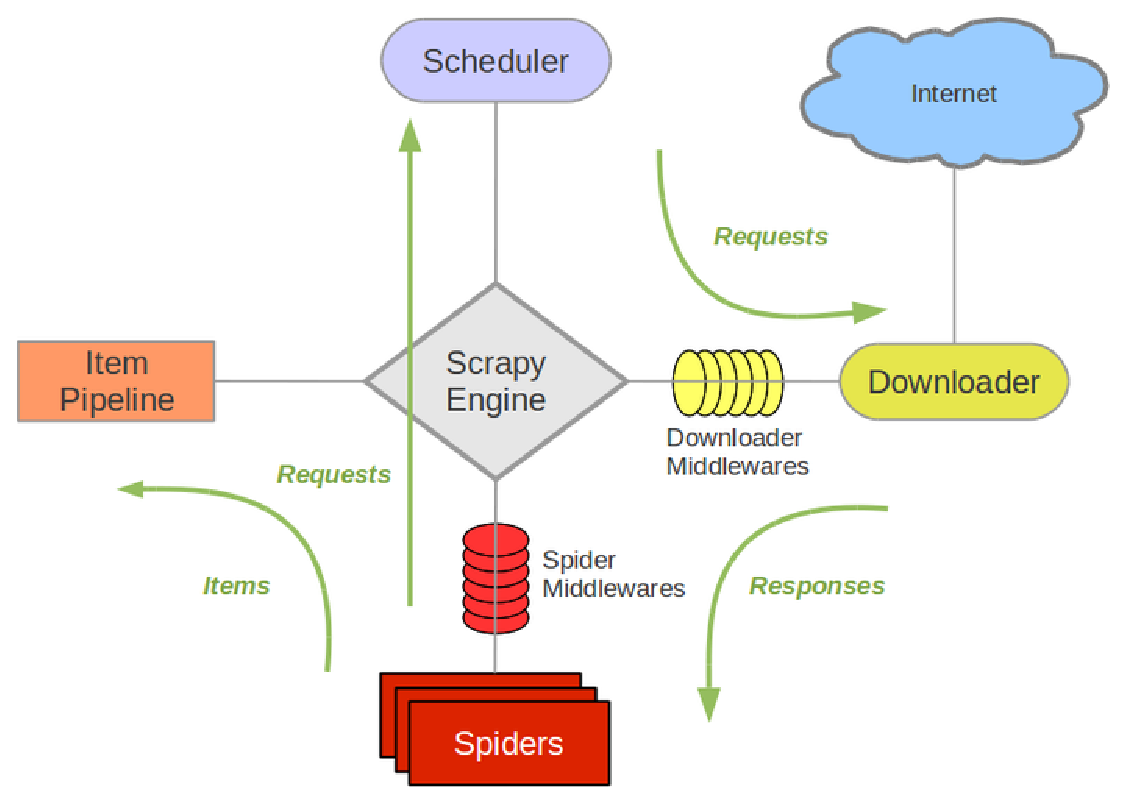
\includegraphics[width=0.47\textwidth]{scrapy_architecture}
  \caption{Overview of the crawler architecture.\\(Credit: Pablo Hoffman, Daniel Graña, Scrapy$^1$)} % Could not found a way...
  \label{scrapyarchitecture}
\end{figure}


%%%%%%%%%%%%%%%%%%%%%%%%%%%%%
\subsection{Enriching Scrapy}\label{enrichingscrapy}

In order to identify web pages as blog posts, our implementation enriches Scrapy with two components to narrow the extraction process down to the subsets of pages which are blog posts: \emph{blog post identification} and \emph{download priority heuristic}.

Given a URL entry point to a website, the default Scrapy behaviour traverses all the pages of the same domain in a \emph{last-in-first-out} manner. The \emph{blog post identification} function is able to identify whether an URL points to a blog post or not. Internally, for each blog, this function uses a regular expression constructed from the blog post URLs found in the web feed. This simple approach requires that blogs use the same URL pattern for all their posts (or false negatives will occur) which has to be distinct for pages that are not posts (or false positives will occur). In practice, this assumption holds for all blog platforms we encountered and seems to be a common practice among web developers.

In order to efficiently deal with blogs that have a large number of pages which are not posts, the \emph{blog post identification} mechanism is not sufficient. Indeed, after all pages identified as blog posts are processed, the crawler needs to download all other pages to search for additional blog posts. To replace the naive \emph{random walk}, \emph{depth first search} or \emph{breadth first search} web site traversals, we use a priority queue where priorities for new URLs are determined by a machine learning system. This mechanism has shown to be mandatory for blogs hosted on a single domain alongside large number of other types of web pages, such as those in forums or wikis.

The idea is to give high priority to URLs which are believed to point to pages with links to blog posts. These predictions are done using an active \emph{Distance-Weighted k-Nearest-Neighbour} classifier \cite{dudani1976}. Let $L(u)$ be the number of links to blog posts contained in a page with URL $u$. Whenever a page is downloaded, its URL $u$ and $L(u)$ are given to the machine learning system as training data. When the crawler encounters a new URL $v$, it will ask the machine learning system for an estimation of $L(v)$, and use this value as the download priority of $v$. $L(v)$ is estimated by calculating a weighted average of the values of the $k$ URLs most similar to $v$.


%%%%%%%%%%%%%%%%%%%%%%%%%%%%%%%%%
\subsection{JavaScript rendering}

JavaScript is a widely used language for client-side scripting. While some applications simply use it for aesthetics, an increasing number of websites use JavaScript to download and display content. In such cases, traditional HTML based crawlers do not see web pages as they are presented to a human visitor by a web browser, and might therefore be obsolete for data extraction.

In our experiments whilst crawling the blogosphere, we encountered several blogs where crawled data was incomplete because of the lack of JavaScript interpretation. The most frequent cases were blogs using the Disqus\footnote{\url{http://disqus.com/websites}} and LiveFyre \footnote{\url{http://web.livefyre.com}} comment hosting services. For webmasters, these tools are very handy because the entire comments infrastructure is externalized and their setup essentially comes down to including a JavaScript snippet in each target page. Both of these services heavily rely on JavaScript to download and display the comments, even providing functionalities such as real-time updates for edits and newly written comments. Less commonly, some blogs are fully rendered using JavaScript. When loading such websites, the web browser will not receive the page content as an HTML document, but will instead have to execute JavaScript code to download and display the page content. The Blogger platform provides the \emph{Dynamic Views} as a default template, which uses this mechanism \cite{antinharasymiv2011}.

To support blogs with JavaScript-generated content, we embed a full web browser into the crawler. After considering multiple options, we opted for PhantomJS\footnote{\url{http://phantomjs.org}}, a headless web browser with great performance and scripting capabilities. The JavaScript rendering is the very first step of web page processing. Therefore, extracting blog post articles, comments or multimedia files works equally well on blogs with JavaScript-generated content and on traditional HTML-only blogs.

When the number of comments on a page exceeds a certain threshold, both Disqus and LiveFyre will only load the most recent ones and the stream of comments will end with a \emph{Show More Comments} button. As part of the page loading process, we instruct PhantomJS to repeatedly click on these buttons until all comments are loaded. Paths to Disqus and LiveFyre \emph{Show More} buttons are manually obtained. They constitute the only non-generic elements of our extraction stack which require human intervention to maintain and extend to other commenting platforms.

%%%%%%%%%%%%%%%%%%%%%%%%
\subsection{Scalability}
When aiming to work with a large amount of input, it is crucial to build every layer of a system with scalability in mind \cite{thereactivemanifesto2013}. The BlogForever Crawler, and in particular the two core procedures \emph{NewCrawl} and \emph{UpdateCrawl}, are designed to be usable as part of an event-driven, scalable and fault-resilient distributed system.

Heading in this direction, we made the key design choice to have both \emph{NewCrawl} and \emph{UpdateCrawl} as stateless components. From a high-level point of view, these two components are \emph{purely functional}:
%
\newcommand\URL{\text{URL}}
\newcommand\DATE{\text{DATE}}
\newcommand\RECORD{\text{RECORD}}
\begin{equation*}
  \begin{split}
    NewCrawl:    &~ \URL \rightarrow \mathcal{P}(\RECORD)\\
    UpdateCrawl: &~ \URL \times \DATE \rightarrow \mathcal{P}(\RECORD)
  \end{split}
\end{equation*}
%
where $\URL$, $\DATE$ and $\RECORD$ are respectively the set of all URLs, dates and records, and $\mathcal{P}$ designates the power set operator. By delegating all shared mutable state to the back-end system, web crawler instances can be added, removed and used interchangeably.
